\begin{center}
Problema I

Campo de Abóboras

{\tiny Por Athos José}

Timelimit: $2$	
\end{center}

Todos os anos varias pessoas participam do Abóbora Contest e neste ano tivemos o ilustre e novo participante Athos. Como principiante, ele plantou vários covas de abóboras sem saber ao certo quantas covas era necessário para ter uma quantidade razoável de abóboras para a competição.

Olhando para o campo por cima, vemos que ele está disposto em um formato de matriz $ N$x$M $, onde cada cova seria uma posição da matriz que possui uma quantidade de abóboras.

Dito isso, Athos pediu para você que responde-se $ Q $ perguntas para ele, as pergunta é dizer quantas abóboras há de um ponto A ao ponto B, sendo A e B posições do campo, ambos inclusos.

Por exemplo, dados os campos em disposição de uma matriz $ 5$x$6 $, e os pontos A e B respectivamente sendo $(2,2)$ e $(3,5)$, a pergunta é dizer quantas abóboras haveria na região cinza.

\begin{figure}[h]
    \centering
    \scalebox{0.5339}{
        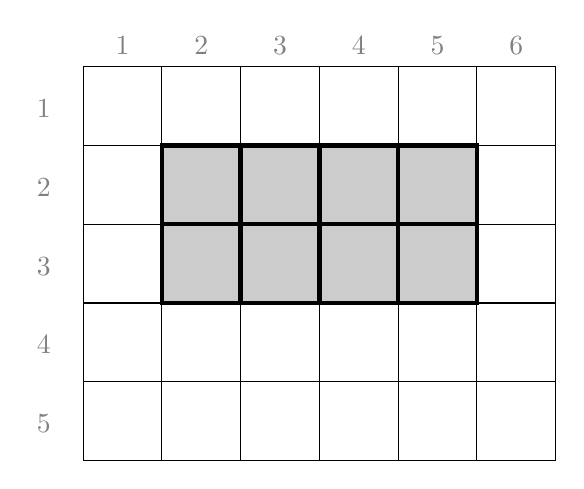
\begin{tikzpicture}
            \foreach \i in {1,...,6} {
                \draw [very thin,gray] node [below] at (\i-0.5,5.5) {$\i$};
            }
            \foreach \i in {1,...,5} {
                \draw [very thin,gray] node [below] at (-0.5,5-\i+0.7) {$\i$};
            }
            \draw[step=1.0,black,thin] (0,0) grid (6,5);
            \draw [ultra thick, draw=black, fill=black!20!white] (1,2) grid  (5,4) rectangle (1,2);
        \end{tikzpicture}
    }
\end{figure}

\vspace{0.3cm}
\textbf{Entrada}

A primeira linha contém três números inteiros $ N $, $ M $ e $ Q $ ($ 1 \leq N, M \leq 10^3 $ e $ 1 \leq Q \leq 3*10^3 $), indicando respectivamente de linhas da matriz, colunas da matriz e o número de perguntas.

Às próximas $ N $ linhas conterá $ M $ valores $ C_{i,j} $ $ (1 \leq C_{ij} \leq 5$ $|$ $1 \leq i \leq N $ e $ 1 \leq j \leq M)$ que é a quantidade de abóbora em cada cova.

Às próximas $Q$ linhas contem 4 números inteiros que são às coordenadas do A e B $(1 \leq A_x \leq B_x \leq N)$ e $(1 \leq A_y \leq B_y \leq M)$.

\vspace{0.3cm}
\textbf{Saída}

A saída deve conter apenas números para cada pergunta feita sendo ele a quantidade de abóboras de A à B.

\begin{table}[ht]
    \centering
    \begin{tabular}{|p{7cm}|p{7cm}|}
        \hline
        \begin{center}
            \vspace{-0.3cm}
            \textbf{Exemplos de Entrada}
            \vspace{-0.3cm}
        \end{center} 
         &  
        \begin{center}
            \vspace{-0.3cm}
            \textbf{Exemplos de Saída}
            \vspace{-0.3cm}
        \end{center} \\ \hline
         \texttt{5 6 4} & \texttt{25} \\  
         \texttt{1 5 4 3 2 1} & \texttt{45} \\
         \texttt{1 2 3 4 5 2} & \texttt{28} \\
         \texttt{2 1 4 3 3 5} & \texttt{90} \\
         \texttt{4 1 5 2 4 3} & \texttt{5} \\
         \texttt{4 3 2 5 5 1} & \texttt{} \\
         \texttt{2 2 3 5} & \texttt{} \\
         \texttt{1 1 4 4} & \texttt{} \\
         \texttt{2 3 5 4} & \texttt{} \\
         \texttt{1 1 5 6} & \texttt{} \\
         \texttt{2 5 2 5} & \texttt{} \\
         \hline
    \end{tabular}
    \caption{Exemplos de entradas e saídas}
    \label{tab:inputN}
\end{table}

\newpage 

\begin{center}
\noindent
\lstinputlisting{abobora_22/I/I2.cpp}
\end{center}